\subsection{Die Ganzen Zahlen}
Symbol: $\mathbb{Z}$\\
sind alle Ganzen Zahlen Positiv als auch Negatiev

\hfill \break
\hfill \break
$ \mathbb{Z}=\{\ldots,-3,-2,-1,0,1,2,3,\ldots\} $

\hfill \break
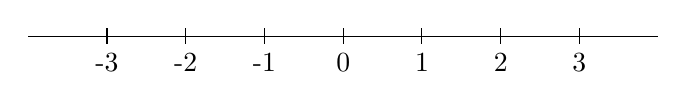
\begin{tikzpicture}
    \draw (-4,0) -- (4,0);
    \foreach \X in {-3,...,3}
    \draw (\X,0.1) -- (\X,-0.1);
    \foreach \X in {-3,-2,-1,0,1,2,3}
    \node[anchor=north] at (\X,-0.1){\X};
\end{tikzpicture}

\hfill \break
Möglichkeiten mit den Ganzen Zahlen:
\begin{enumerate}
    \item Subtrahieren ist uneingeschränkt möglich:
          \begin{itemize}
              \item 1-3 = -2
              \item 10-5 = 5
          \end{itemize}
    \item Dividieren ist nur eingeschränkt möglich:
          \begin{itemize}
              \item 1/3 = ?
              \item 10/5 = 2
          \end{itemize}
\end{enumerate}